\documentclass{beamer}
\usepackage[utf8]{inputenc}
\usepackage{polski}
\usepackage{graphics}
\usepackage{wrapfig}
\usepackage{subfig}
\setbeamercovered{transparent}
\usetheme{Warsaw}
\usepackage{color}
\title[Dalsze plany pewnego studenta]{Co będę robił w następnym semestrze?!?!?!}
\author{Piotr Piesiak}
\date{January 22, 2041}
\begin{document}

\begin{frame}
\titlepage
\end{frame}


\begin{frame}{Przedmioty}

\begin{block}{Przedmioty do wyboru}

\begin{tabular}{|c||c||c|}
\hline
\textbf{Matematyka}& \textbf{Informatyka}& \textbf{Dodatki}\\
\hline
 Algebra I & Metody Programowania & Angielski \\
\hline
 Analiza Matematyczna 2 & Sztuczna inteligencja & Hisotria \\
\hline
\end{tabular}

\end{block}

\visible<1>{W kolejnym semestrze będę musiał wybrać między innymi przedmioty z tabeli}
\begin{itemize}
  \visible<1>{\item Trzeba będzie dokonać wyboru między obowiązkami na danym semestrze oraz obowiązkami informatycznymi lub matematycznymi z przyszłych semestrów - w taki sposób, aby zrównoważyć ilość pracy w kązdym semestrze i uzyskać wymaganą ilość ECTS.}
	\pause 
\item A skoro o ECTS-ach mowa...
  \end{itemize}
\end{frame}

\begin{frame}{ECTS}
\begin{tabular}{ll}
		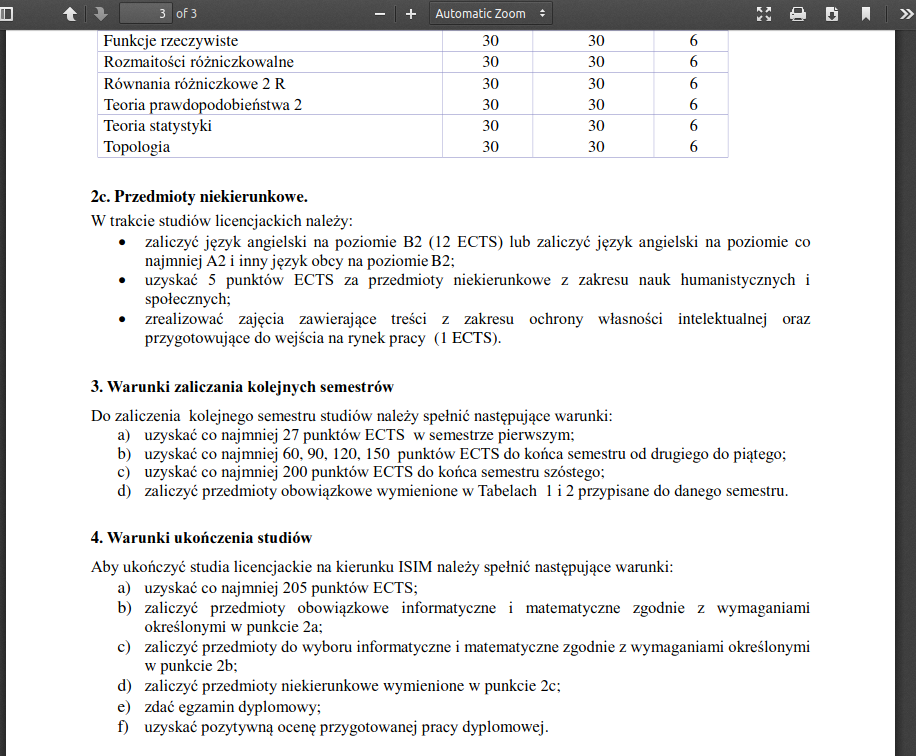
\includegraphics[width=3.5cm,angle=30]{zdj.png} &
		\parbox{0.5\linewidth}{
		\textbf{Szczegółowy opis kierunku} Na zdjęciu widać opisane obowiązki studenta ISIMU. Muszę tak rozłożyć przedmioty, aby do końca semestru 6 uzyskać 200 pkt ECTS. Do tej pory zdobyłem około 36. Poza ECTS-ami trzeba pamiętać o obowiązkowych przedmiotach z wcześniejszych tabelek.}

\end{tabular}

\end{frame}

\begin{frame}{Przedmioty, na których chciałbym się skupić: Algebra}
\begin{columns}
\column{0.5\textwidth}
\begin{figure}
\centering
\subfloat{
	\includegraphics[width=0.4\textwidth]{alg.pdf}
}
\subfloat{
	\includegraphics[width=0.4\textwidth]{alg2.pdf}
}
\end{figure}
\column{0.5\textwidth}
W tym semestrze zaciekawiła mnie Algebra prowadzona przez profesroa Jana Dymarę. W przyszłości chciałbym się na niej skupić - ma bardzo wiele zastosowań w informatyce.
\end{columns}
\end{frame}

\begin{frame}{Przedmioty, na których chciałbym się skupić: Analiza}
\begin{columns}
\column{0.5\textwidth}
Analiza to kolejny przedmiot, który poznam trochę szerzej i głębiej. Jest to istotny przedmiot w dalszej nauce, który potrafi być ciekawy.
\column{0.5\textwidth}
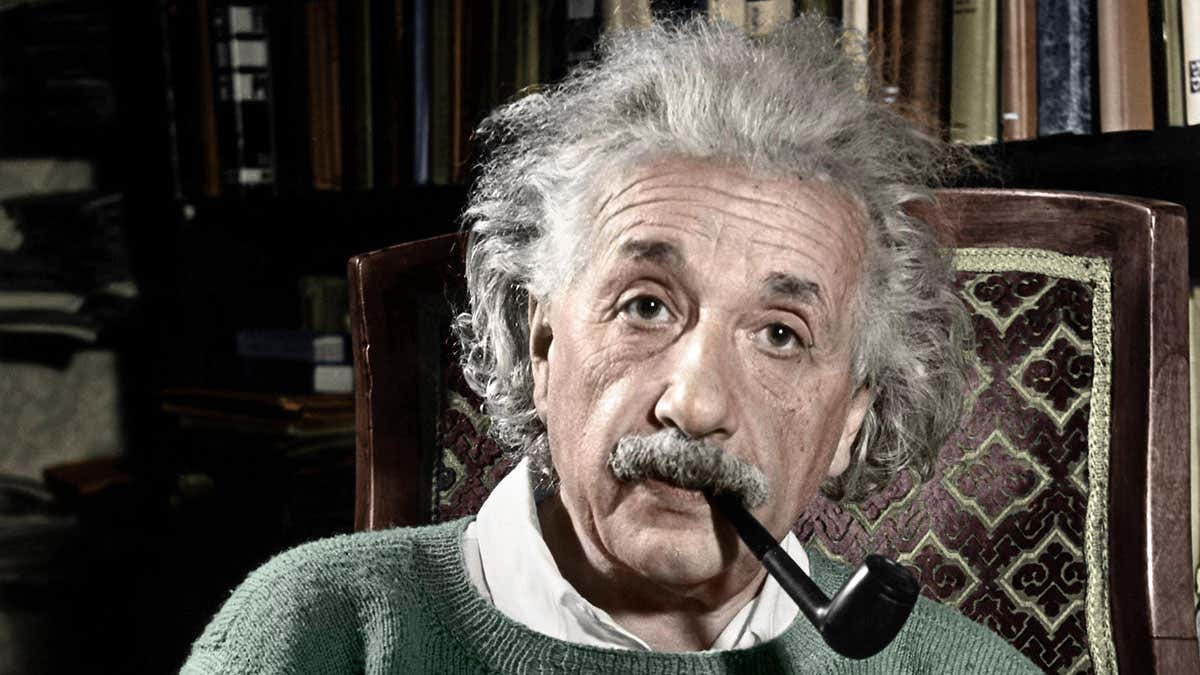
\includegraphics[width=4cm]{zdjj.jpg}
\end{columns}
\end{frame}

\begin{frame}{Urozmaicenie semestry: Angielski}
\begin{columns}
\column{0.5\textwidth}

\includegraphics[width=0.4\textwidth]{ang.jpg}
\newline
Zalety J.Angieslkeigo:
\onslide<1->{Komunikatywność w przyszłości}
 
\onslide<2->{Dostęp do większej ilości filmów}
 
\onslide<3->{Dostęp do większej ilości materiałów}
\column{0.5\textwidth}

\includegraphics[width=0.6\textwidth]{grf.jpg}
\end{columns}

\end{frame}

\begin{frame}{KONIEC}
\begin{block}{JUŻ KONIEC!}
\textbf<2>{Dziękuję za uwagę!}
\begin{tabular}{|r|}
\textrm<2>{Przygotował:} \\
\textcolor<2>{orange}{Piotr}
\textcolor<2>{blue}{Piesiak}
\end{tabular}
\end{block}
\begin{center}

\includegraphics[width=6cm]{memik.jpg}
\end{center}
\end{frame}
\end{document}
